\chapter{Relations, relations d'ordre, d'équivalence. Lois de composition}
\origpage{27--49}

Au chapitre 0, on a introduit la notion de relation mathématique comme étant un assemblage écrit à partir des symboles de la théorie, cet assemblage pouvant être vrai ou non.

Ici nous allons parler de \emph{relation sur un ensemble} et le mot relation aura une autre signification.

\BellaSection{1. Vocabulaire}

\medskip\noindent\textsc{Définition 2.1.} --- \emph{On appelle relation $R$ sur un ensemble $E$ la donnée d'une partie $R$ de $E\times E$. On parle encore de relation binaire car agissant sur des couples.}

On dira que $x$ et $y$, pris dans cet ordre, vérifient $R$, et on note $xRy$, si et seulement si $(x,y)\in R$.

Les différences avec une application de $E$ dans $E$, c'est-à-dire la donnée d'un graphe de $E$, sont les suivantes :
\begin{itemize}[leftmargin=2em]
\item pour un $x$ fixé, il peut y avoir \emph{plusieurs} $y$ de $E$ tels que $(x,y)\in R$, (dans un graphe, il y a un seul $y$ associé à $x$) ;
\item des $x$ de $E$ peuvent ne pas avoir de $y$ associé tel que $(x,y)\in R$.
\end{itemize}

Bien sûr, ce qui intéresse dans la donnée d'une relation sur un ensemble $E$, c'est la formulation du lien entre $x$ et $y$, et non la donnée de l'ensemble $R$.

De même une partie $R$ quelconque du produit cartésien $E\times E$ définit une relation qui a peu de chances d'être intéressante, aussi va-t-on définir d'autres termes.

\subsection*{2.2.}
Une relation $R$ sur $E$ est dite \emph{réflexive} si et seulement si, pour tout $x$ de $E$, on a $xRx$ ; elle est dite \emph{symétrique} si et seulement si, quand $xRy$ on a aussi $yRx$. Enfin elle est dite \emph{transitive} si et seulement si $(xRy)$ et $(yRz)$ impliquent $(xRz)$.

Une relation est dite \emph{antisymétrique} si et seulement si $(xRy)$ et $(yRx)$ impliquent $x=y$.

\BellaSection{2. Relation d'équivalence sur un ensemble}

\medskip\noindent\textsc{Définition 2.3.} --- \emph{On appelle relation d'équivalence sur un ensemble $E$ toute relation $R$ sur $E$ qui est réflexive, symétrique et transitive.}

Autrement dit, toute relation $R$ vérifiant les conditions suivantes :
\begin{enumerate}[label=\arabic*)]
\item $\forall x\in E$, $xRx$ ;
\item $\forall(x,y)\in E\times E$ tel que $xRy$, on a $yRx$ ;
\item si $x,y,z$ sont dans $E$ et si on a $(xRy)$ et $(yRz)$ alors on a $(xRz)$.
\end{enumerate}

\medskip\noindent\textsc{Exemple 2.4.} --- $E=\mathbb Z$, ensemble des entiers relatifs, (qui sera construit par la suite, mais que l'on connaît en fait). Si on se donne un entier naturel $p$, non nul, la relation $R_p$ définie par
\[
xR_py\Leftrightarrow x-y\text{ est divisible par }p
\]
est une équivalence (vérification laissée au lecteur) appelée \emph{congruence modulo $p$}.

On a
\[
xR_py\Leftrightarrow\exists q\in\mathbb Z,\quad x-y=pq,
\]
et avec cette formulation, il est facile de vérifier \BellaCorrection{réflexivité}{réflexiviste}, symétrie, transitivité. \bookend

Les relations d'équivalence vont conduire à un mécanisme fondamental en mathématiques : celui du « passage au quotient » qui est la formulation mathématique d'une démarche humaine. Je m'explique : soit l'ensemble des humains, (on ne fait plus des mathématiques, ici le vocabulaire a son sens conventionnel) et la relation $N$ définie par
\[
xNy\Leftrightarrow x\text{ et }y\text{ ont la même nationalité},
\]
(on suppose qu'il n'y a pas de nationalités multiples).

Cette relation $N$ est réflexive, symétrique et transitive, et elle permet de « classer » les humains par nations, (les Français ensemble, les Anglais aussi...) Du point de vue des nations, ce ne sont plus les individus que l'on considère, mais les groupements d'individus de même nationalité.

\subsection*{2.5. Ensemble quotient}

Soit $R$ une relation d'équivalence sur un ensemble $E$.

Soit $x\in E$, on considère la partie $\mathcal X$ de $E$ définie par
\[
y\in\mathcal X\Leftrightarrow xRy.
\]
Cette partie qui est non vide, (car $xRx\Rightarrow x\in\mathcal X$) s'appelle la \emph{classe d'équivalence de $x$}. Elle est formée de l'ensemble des $y$ équivalents à $x$.

À chaque $x$ de $E$ on peut associer sa classe d'équivalence, $\mathcal X$.

La réunion des classes d'équivalence donne $E$ entier : car $\forall a\in E$, $a\in\mathcal A$ classe de $a$, donc
\[
a\in\bigcup_{x\in E}\mathcal X
\]
en notant toujours $\mathcal X$ la classe de $x$, car parmi les parties $\mathcal X$ figure $\mathcal A$. \bookend

Deux classes distinctes sont disjointes : supposons que $\mathcal A$, classe de $a$ et $\mathcal B$ classe de $b$ contiennent un élément commun, $c$.

Soit $x\in\mathcal A$, comme $c\in\mathcal A$ aussi, on a $xRa$ et $cRa$ donc $aRc$, (symétrie de $R$), mais alors $(xRa\text{ et }aRc)\Rightarrow xRc$.

Mais $c\in\mathcal B$ classe de $b$ : on a donc $bRc$, (définition de $\mathcal B$), d'où $cRb$, (symétrie), mais alors $(xRc)$ et $(cRb)\Rightarrow(xRb)$, (transitivité de $R$) : donc $x$ étant équivalent à $b$, est dans la classe de $b$. On a prouvé que, $\forall x\in\mathcal A$, $x\in\mathcal B$, soit encore $\mathcal A\subset\mathcal B$. Par analogie des rôles joués on a aussi $\mathcal B\subset\mathcal A$. Donc
\[
\mathcal A\cap\mathcal B\ne\varnothing\Rightarrow\mathcal A=\mathcal B :
\]
par contraposée, si $\mathcal A$ et $\mathcal B$ sont distinctes elles sont disjointes, c'est-à-dire d'intersection vide.

\subsection*{2.6. Partition}

Les différentes classes d'équivalence des éléments de $E$ sont des parties de $E$, non vides, disjointes, dont la réunion donne $E$. On dit alors que ces classes d'équivalence forment une \emph{partition} de $E$, et la partie de $\mathcal P(E)$, (ensemble des parties de $E$), dont les éléments sont les classes d'équivalence s'appelle \emph{l'ensemble quotient} de $E$ par $R$, noté $E/R$.

En fait, on a ici la clé de la construction des ensembles mathématiques intéressants : on construira $\mathbb Z$ à partir de $\mathbb N$ en établissant une équivalence sur $\mathbb N\times\mathbb N$ ; $\mathbb Q$ à partir de $\mathbb Z$, $\mathbb R$ à partir de $\mathbb Q$, $\mathbb C$ à partir de $\mathbb R$ en utilisant à chaque fois des passages aux ensembles quotients.

Il faut noter que, si on part d'une partition de l'ensemble $E$ c'est-à-dire d'une famille $\mathcal F$ de parties de $E$ qui sont non vides, disjointes, de réunion $E$, et si on définit la relation $R$ par
\[
(xRy)\Leftrightarrow(x\text{ et }y\text{ sont dans la même partie }A\text{ de }E,\ A\in\mathcal F),
\]
on a une équivalence.

Notons $(F_i)_{i\in I}$ la famille $\mathcal F$, (l'intérêt de l'indexation apparaît dans cette façon de noter).

On a $R$ réflexive car, comme $\bigcup_{i\in I}F_i=E$, à chaque $x\in E$ on associe au moins un $i_0\in I$ tel que $x\in F_{i_0}$, donc $x$ et $x$ sont dans la même $F_{i_0}$ : on a $xRx$ ;

$R$ est symétrique : si $xRy$, c'est que $x$ et $y$ sont dans une même partie $F_i$ de la famille $\mathcal F$, donc $y$ et $x$ aussi, donc $yRx$ ;

$R$ est transitive : si $xRy$ et $yRz$, c'est que $x$ et $y$ sont dans une même partie $F_{i_1}$, et que $y$ et $z$ sont dans une même partie disons $F_{i_2}$, or si $F_{i_1}\ne F_{i_2}$ on a $F_{i_1}\cap F_{i_2}=\varnothing$, (parties disjointes) donc comme $y\in F_{i_1}\cap F_{i_2}$ c'est que $F_{i_1}=F_{i_2}$ : $x$ et $z$ sont dans cette partie $F_{i_1}$ d'où $xRz$. On a bien une équivalence. \bookend

Si $R$ est une relation d'équivalence, l'application $p$ de $E$ sur l'ensemble quotient $E/R$ qui à un élément $x$ de $E$ \BellaCorrection{associe}{associé} sa classe d'équivalence, $p(x)$, (souvent notée $\bar x$ ou $\mathcal X$ ou $F_x$...), s'appelle \emph{l'application canonique} de $E$ sur $E/R$ : elle est surjective, puisque chaque classe d'équivalence $F$ étant non vide, n'importe quel $x$ de $F$ est envoyé par $p$ sur $F$, et $x$ s'appelle un \emph{représentant} de la classe $p(x)$.

Si on reprend l'exemple, (mauvais), des nations, la « classe d'équivalence » nation des français est représentée par n'importe quel français choisi dans cette classe...

\BellaSection{3. Relation d'ordre}

\medskip\noindent\textsc{Définition 2.7.} --- \emph{On appelle \BellaCorrection{relation d'ordre}{d'ordre}, sur un ensemble $E$, toute relation réflexive, antisymétrique et transitive.}

Habituellement on notera $x\le y$ au lieu de $xRy$, la relation d'ordre qui se lit « $x$ inférieur ou égal à $y$ ».

Dire que $\le$ est un ordre sur $E$ équivaut donc à dire que
\begin{align*}
&1)\quad \forall x\in E,\ x\le x &&\text{(réflexivité)};\\
&2)\quad \forall(x,y)\in E^2,\ ((x\le y)\text{ et }(y\le x))\Rightarrow x=y &&\text{(antisymétrie)};\\
&3)\quad \forall(x,y,z)\in E^3,\ ((x\le y)\text{ et }(y\le z))\Rightarrow x\le z &&\text{(transitivité)}.
\end{align*}

\medskip\noindent\textsc{Exemple 2.8.} --- Il est facile de voir que la relation d'inclusion sur l'ensemble $\mathcal P(E)$ des parties de $E$ est une relation d'ordre sur $\mathcal P(E)$.

\medskip\noindent\textsc{Exemple 2.9.} --- Sur $\mathbb N$, la relation
\[
(x\ge y)\Leftrightarrow(\exists z\in\mathbb N,\ x=y+z),
\]
est aussi une relation d'ordre. (Justification laissée au lecteur éventuel).

\medskip\noindent\textsc{Remarque 2.10.} --- Il y a une différence entre les 2 exemples : dans le 1\textsuperscript{er} cas, étant données 2 parties $A$ et $B$ de $E$ on peut ne pas avoir $A\subset B$ ou $B\subset A$, c'est-à-dire, avoir $A$ et $B$ non comparables : l'ordre est dit \emph{non total} dans ce cas, (alors que dans l'exemple 2, deux entiers étant donnés, l'un est supérieur ou égal à l'autre : l'ordre est alors \emph{total}).

\medskip\noindent\textsc{Remarque 2.11.} --- Il arrive que l'on parle de \emph{relation d'ordre strict} pour \BellaCorrection{une relation}{un relation} $R$ qui est \BellaCorrectionNote{irréflexive et transitive}{antisymétrique et transitive}{Pour un ordre strict, l'antisymétrie ne suffit pas : une relation d'ordre large comme $\le$ est antisymétrique et transitive sans être stricte. La formulation standard exige l'irréflexivité et la transitivité (équivalemment, l'asymétrie et la transitivité).}, on notera $\prec$ ou $\succ$ une telle relation.

\subsection*{Élément maximal, minimal, maximum, minimum}

Soit un ensemble ordonné $E$, la relation d'ordre étant \BellaCorrection{notée}{noté} $\le$.

\subsection*{2.12.}
Un élément $a$ est dit maximal
\[
\Leftrightarrow (\nexists x\in E,\ x\succ a),
\]
ou encore
\[
\Leftrightarrow \forall y\in E-\{a\},\quad
\begin{cases}
\text{soit }y\text{ et }a\text{ non comparables},\\
\text{soit }y\le a.
\end{cases}
\]

\subsection*{2.13.}
Un élément $m$ est dit maximum
\[
\Leftrightarrow(\forall x\in E,\ x\le m).
\]
De tels éléments n'existent pas forcément : dans $\mathbb N$, pour l'ordre usuel, il n'y a pas d'élément maximal ni maximum. Par contre dans $\mathcal P(E)$ ordonné par inclusion $E$ est visiblement maximum.

\medskip\noindent\textsc{Remarque 2.14.} --- Si $E$ ordonné admet un élément maximum, $m$, il est unique. Car si $m'$ est aussi maximum, on a $m\ge m'$ car $m$ maximum est supérieur ou égal à tout élément, et $m'\ge m$ car $m'$ maximum d'où $m=m'$ par antisymétrie. \bookend

Par contre, il peut y avoir plusieurs éléments maximaux.

\medskip\noindent\textsc{Exemple 2.15.} --- $E=\{2,3,\ldots,20\}$, on définit $R$ par $aRb\Leftrightarrow a$ divise $b$, c'est visiblement réflexif, antisymétrique, transitif, donc on a une relation d'ordre, et dans $E$, les \BellaCorrection{nombres}{nombre} $11,12,13,\ldots,20$ sont maximaux.

\medskip\noindent\textsc{Remarque 2.16.} --- Si $E$ totalement ordonné et s'il y a un élément maximal, il est unique. Si $a$ et $b$ sont chacun maximal, étant comparables ($E$ totalement ordonné) on a $a\le b$ ($b$ maximal) et $b\le a$, ($a$ maximal), d'où $a=b$, (antisymétrie de l'ordre). \bookend

De plus cet unique élément maximal est maximum puisque, tout $x$ de $E$ étant comparable à $a$ maximal, on a forcément $x\le a$.

\subsection*{2.17.}
On définit de même les termes suivants : $a$ minimal $\Leftrightarrow$ il n'existe pas de $x$ dans $E$ tel que $x\ne a$ et $x\le a$, (on pourrait noter $\nexists x\in E$, $x\prec a$, si $\prec$ est l'ordre strict).

\subsection*{2.18.}
On dit que $a$ est minimum dans $E\Leftrightarrow\forall x\in E$, $x\ge a$.

\subsection*{2.19.}
Si $A$ est une partie de $E$ ensemble ordonné, on dit que $A$ est \emph{majorée} (resp. \emph{minorée}) s'il existe $m$ dans $E$ tel que $\forall x\in A$, $x\le m$ (resp. $x\ge m$) et dans ce cas $m$ s'appelle un \emph{majorant} de $A$, (resp. un \emph{minorant}).

Il faut remarquer que $m$ n'est pas forcément dans $A$, (exemple : dans $\mathbb R$, $A=\{1-\frac1n;\ n\in\mathbb N^*\}$ est majorée par $1$, $1\notin A$, et il n'y a pas de majorant plus petit que $1$).

Cependant, si le majorant $m$ de $A$ est dans $A$, dans ce cas c'est le \emph{plus petit majorant}. On appelle plus petit majorant, l'élément $m$, s'il existe qui majore $A$ et tel que $\forall m'$ majorant de $A$ on ait $m\le m'$. Si un tel élément existe il est unique car si $m_1$ et $m_2$ sont plus « petit majorant de $A$ », on a $m_1\le m_2$ car $m_1$ plus petit majorant et $m_2\le m_1$ car $m_2$ plus petit majorant, d'où $m_1=m_2$ par \BellaCorrection{antisymétrie}{antisymétrique} de la relation d'ordre. \bookend

\subsection*{2.20.}
On appelle encore \emph{borne supérieure} de $A$ (resp. \emph{inférieure}) le plus petit majorant (resp. grand minorant) de $A$, s'il existe, et un ensemble est dit \emph{borné} s'il admet des majorants et des minorants. On notera $\sup A$ (resp. $\inf A$) cet élément, s'il existe. Attention, le plus souvent ce ne sont pas des éléments de $A$.

\BellaSection{4. Morphismes, loi de composition}

\medskip\noindent\textsc{Définition 2.21.} --- \emph{Soient $E$ et $F$ deux ensembles munis de relations binaires notées $R$ et $S$ respectivement, et $f$ une application de $E$ dans $F$. On dit que $f$ est compatible avec $R$ et $S$, (ou encore que $f$ est un morphisme pour $R$ et $S$) si et seulement si :}
\[
\forall(x,y)\in E^2,\qquad xRy\Rightarrow f(x)Sf(y).
\]

\subsection*{2.22.}
Si $F=E$, on parle d'endomorphisme ; si $f$ est bijective et si $f^{-1}$ application réciproque de $F$ sur $E$ est aussi un morphisme, on parle d'isomorphisme, et d'automorphisme si de plus $E=F$.

\subsection*{2.23. Transport de structure}
Soient $E$ et $F$ deux ensembles, $f$ une bijection de $E$ sur $F$. Si on suppose $E$ muni d'une relation $R$, on peut définir une relation $\widetilde R$ sur $F$ par :
\[
\forall(y,y')\in F^2,\qquad y\widetilde R y'\Leftrightarrow f^{-1}(y)R f^{-1}(y'),
\]
($f^{-1}(y)$ et $f^{-1}(y')$ étant les antécédents, dans $E$, de $y$ et $y'$), et le côté bijectif de $f$ permet de voir que $\widetilde R$ sera réflexive (ou symétrique, antisymétrique, transitive...) si et seulement si $R$ l'est donc $R$ équivalence $\Leftrightarrow\widetilde R$ l'est ; il en est de même pour une relation d'ordre : on transporte la structure sur $E$ liée à $R$ sur l'ensemble $F$, et pour $R$ et $\widetilde R$, $f$ devient un isomorphisme. \bookend

Cette notion de morphisme va se retrouver avec les lois de composition.

\medskip\noindent\textsc{Définition 2.24.} --- \emph{Soit un ensemble $E$. On appelle loi de composition interne sur $E$ toute application de $E\times E$ dans $E$.}

Il s'agit donc d'une notion déjà connue, mais que l'on va noter différemment par commodité. Au lieu de noter :
\[
f:E\times E\longmapsto E,\qquad\text{ou}\qquad (x,y)\longmapsto z=f(x,y),
\]
on utilise un symbole, ($+$, $\times$, $*$, $\wedge$, $\top$, $\perp$, $\otimes$, $\oplus$,...) disons ici $*$ par exemple, pour noter l'image du couple $(x,y)$ sous la forme $z=x*y$.

La loi interne est dite :

\subsection*{2.25.}
commutative $\Leftrightarrow\forall(x,y)\in E^2$, $x*y=y*x$,

\subsection*{2.26.}
associative $\Leftrightarrow\forall(x,y,z)\in E^3$, $x*(y*z)=(x*y)*z$.

Par exemple, sur $\mathbb N^*$, la loi $a*b=a^b$ n'est pas commutative car $2^3=8\ne3^2=9$, ni associative $2^{(2^3)}=2^8=256$ alors que $(2^2)^3=4^3=64$.

\subsection*{2.27.}
Un élément $i$ de $E$ est dit \emph{idempotent} pour la loi $*$ si on a :
\[
i*i=i.
\]

\subsection*{2.28.}
Un élément $e$ de $E$ est dit
\begin{align*}
&\text{neutre à gauche si }\forall x\in E,\ e*x=x,\quad(e\text{ est à gauche}),\\
&\text{neutre à droite si }\forall x\in E,\ x*e=x,\\
&\text{neutre s'il est neutre à droite et à gauche.}
\end{align*}
Pour la loi précédente $1$ est neutre à droite car $a*1=a^1=a$, mais pas à gauche car $1*a=1^a=1$ et pas $a$.

\medskip\noindent\textsc{Théorème 2.30.} --- \emph{Si dans $E$ muni d'une loi de composition, notée $*$, il existe un élément neutre à droite, $e$, et un élément neutre à gauche, $e'$, on a forcément $e=e'$.}

Car $e$ neutre à droite $\Rightarrow e'*e=e'$, et $e'$ neutre à gauche $\Rightarrow e'*e=e$, d'où $e'=e$. \bookend

Donc s'il y a un élément neutre, (des 2 côtés) il est unique, mais il peut y avoir
\begin{center}
plusieurs neutres à droite, (et pas de neutre à gauche),\\
ou plusieurs neutres à gauche, (et pas de neutre à droite).
\end{center}

\subsection*{2.31. Inverses}

Soit un ensemble $E$ muni d'une loi de composition interne, $*$, ayant un élément neutre $e$, (des 2 côtés).

On dit que $x$ admet un inverse à droite, $x'$, si on a $x*x'=e$, et de même $x$ admet un inverse à gauche, $x''$, si on a $x''*x=e$.

On dit que $x$ admet un inverse $x'$ si on a à la fois $x*x'=e$ et $x'*x=e$.

Bien sûr, si la loi est commutative, les notions de droite et de gauche n'ont plus de signification. A quand la politique commutative ?

\medskip\noindent\textsc{Théorème 2.32.} --- \emph{Soit $E$ un ensemble muni d'une loi de composition interne $*$, associative et ayant un élément neutre. Si un élément $x$ admet un inverse à droite, $x'$, et un à gauche, $x''$, on a $x'=x''$.}

Car $x''*(x*x')=x''*(e)=x''$, et par associativité, c'est aussi $(x''*x)*x'=e*x'=x'$ d'où $x'=x''$. \bookend

C'est pourquoi, de tels ensembles, appelés demi-groupes unitaires, sont appelés à un riche avenir : nous le retrouverons dans l'étude des groupes.

\subsection*{Distributivité 2.33.}
Si sur un ensemble $E$ on a 2 lois de composition interne, $*$ et $\perp$, on dit que $\perp$ est distributive à gauche pour la loi $*$ si on a
\[
\forall(x,y,z)\in E^3,\qquad x\perp(y*z)=(x\perp y)*(x\perp z).
\]
En quelque sorte, la loi $\perp$ distribue son action sur chacun des 2 éléments $y$ et $z$. On parle de même de distributivité à droite et de distributivité si c'est des 2 côtés.

\medskip\noindent\emph{Loi de composition externe.} (sera utilisée dans les espaces vectoriels).

\medskip\noindent\textsc{Définition 2.34.} --- \emph{\BellaCorrection{Soient deux ensembles}{Soit deux ensemble} $K$ et $E$. On appelle loi de composition externe sur $E$, associée à l'ensemble $K$, toute application de $K\times E$ dans $E$. On dit que les éléments de $K$ sont les opérateurs.}

C'est ainsi que si $K$ est un corps, ($K=\mathbb R$ par exemple), sur un espace vectoriel $E$ on définira le produit d'un vecteur $V$ par un scalaire $\lambda\in K$, donc une application de $K\times E\longmapsto E$ qui au couple $(\lambda,V)$ de $K\times E$ associera un vecteur noté $\lambda\cdot V$ ou $\lambda V$.

On peut alors donner un deuxième sens au terme morphisme :

\medskip\noindent\textsc{Définition 2.35.} --- \emph{\BellaCorrection{Soient deux ensembles}{Soit deux ensembles} $E$ et $E'$ munis de lois de composition interne notées respectivement $T$ et $T'$ et $f$ une application de $E$ dans $E'$. On dit que $f$ est un morphisme de $(E,T)$ dans $(E',T')$ si et seulement si}
\[
\forall(x,y)\in E^2,\qquad f(xTy)=f(x)T'f(y).
\]
Ou plus brièvement : « l'image du composé est le composé des images ».

On introduit encore les termes d'isomorphisme, d'endomorphisme et d'automorphisme, ainsi que la notion de transport de structure, comme pour les relations binaires.

Enfin, si $E$ et $E'$ sont deux ensembles munis de lois de composition externe $\perp$, $\perp'$, ayant le même ensemble $K$ d'opérateurs, on dit que $f:E\to E'$ est un morphisme si on a :
\[
\forall(\lambda,x)\in K\times E,\qquad f(\lambda\perp x)=\lambda\perp' f(x).
\]

Il est facile de vérifier que, si $E$ et $E'$ sont 2 ensembles munis de lois internes $T$ et $T'$, et si $f:E\to E'$ est un morphisme surjectif : alors
\begin{enumerate}[label=\arabic*)]
\item $T$ commutative $\Rightarrow T'$ commutative ;
\item $T$ associative $\Rightarrow T'$ associative ;
\item $e$ neutre pour $T\Rightarrow f(e)$ neutre pour $T'$ ;
\item $x'$ inverse de $x$ pour $T\Rightarrow f(x')$ inverse de $f(x)$ pour $T'$.
\end{enumerate}
Le 3) et 4) peuvent se formuler avec « à droite » ou « à gauche ».

Justifions 3) par exemple, (les autres justifications sont laissées au lecteur).

Pour tout $z'\in E'$, $\exists x\in E$, $f(x)=z'$ car $f$ surjective, donc
\begin{align*}
z'T'f(e)&=f(x)T'f(e)\\
&=f(xTe)\text{ car }f\text{ morphisme},\\
&=f(x)\text{ car }e\text{ neutre pour }T,\\
&=z',
\end{align*}
et de même
\[
f(e)T'z'=f(e)T'f(x)=f(eTx)=f(x)=z'.
\]
Finalement, $\forall z'\in E'$ on a bien $z'T'f(e)=f(e)T'z'=z'$, $f(e)$ est neutre dans $E'$ pour la loi $T'$.

Il ne faut cependant pas croire que toute propriété d'une loi de composition interne se conserve par morphisme surjectif.

Considérons par exemple la notion de régularité.

\subsection*{2.36.}
Sur l'ensemble $E$ muni de la loi $T$, un élément $x$ est dit \emph{régulier à droite} sur $E$ si on a :
\[
\forall(y,z)\in E^2,\qquad(yTx=zTx)\Rightarrow y=z.
\]
S'il en est ainsi, et si $f$ est un morphisme surjectif de $E$ sur $E'$ muni de $T'$ on n'a pas forcément $f(x)$ régulier à droite car :
\[
\forall(y',z')\in E'^2,\quad\text{avec }(y,z)\in E^2\text{ tel que }f(y)=y'\text{ et }f(z)=z',
\]
l'égalité $y'T'f(x)=z'T'f(x)$ s'écrit encore
\[
f(y)T'f(x)=f(z)T'f(x),
\]
soit $f(yTx)=f(zTx)$ puisque $f$ est un morphisme et... c'est tout car si $f$ est non injective, on ne peut rien dire de plus.

\medskip\noindent\textsc{Théorème 2.37.} --- \emph{Soient $E$ et $E'$ deux ensembles munis de lois de composition interne $T$ et $T'$ et $\varphi$ un morphisme bijectif de $E$ sur $E'$. Alors l'application réciproque $\varphi^{-1}$ est aussi un morphisme.}

On veut prouver que :
\[
\forall(x',y')\in E'^2,\qquad \varphi^{-1}(x'T'y')=\varphi^{-1}(x')T\varphi^{-1}(y').
\]
Comme $\varphi$ est bijective, ceci équivaut à ce que les images des deux membres de l'égalité, par $\varphi$, soient égales.

Or
\[
\varphi\bigl(\varphi^{-1}(x'T'y')\bigr)=x'T'y',
\]
alors que, $\varphi$ étant un morphisme,
\begin{align*}
\varphi\bigl(\varphi^{-1}(x')T\varphi^{-1}(y')\bigr)
&=\varphi(\varphi^{-1}(x'))T'\varphi(\varphi^{-1}(y'))\\
&=x'T'y'.
\end{align*}
On a bien l'égalité voulue. \bookend

Ce résultat justifié pour un morphisme pour des lois de composition ne s'étend pas pour un morphisme pour des relations binaires $R$ et $R'$ sur $E$ et $E'$, car le fait que $x'R'y'$ dans $E'$ n'implique pas que les antécédents $x=f^{-1}(x')$ et $y=f^{-1}(y')$ soient en relation avec $R$. Il y a des cas où le résultat est valable, par exemple celui d'ordres totaux sur $E$ et $E'$.

\subsection*{2.38. Factorisation des morphismes}

Soit $E$ muni d'une loi de composition, notée $*$, et $R$ une relation binaire sur $E$. On dit que $R$ est compatible avec la loi interne $*$ si et seulement si
\[
xRx'\text{ et }yRy'\Rightarrow(x*y)R(x'*y').
\]
Ceci est surtout utilisé lorsque $R$ est une équivalence : si elle est compatible avec la loi $*$, on va définir une loi interne, encore notée $*$, sur l'ensemble quotient $E/R$ car, si $\mathcal X$ et $\mathcal Y$ sont deux éléments de $E/R$, c'est-à-dire deux parties de $E$, classes d'équivalence pour $R$, si on prend
\begin{center}
$x$ et $x'$ dans $\mathcal X$ d'une part,\\
$y$ et $y'$ dans $\mathcal Y$ d'autre part,
\end{center}
on a $xRx'$ et $yRy'$ d'où $(x*y)R(x'*y')$. En notant $\mathcal X*\mathcal Y$ la classe d'équivalence de $x*y$, on obtient la même classe en partant de $x'*y'$ : c'est indépendant du choix des représentants $x$ dans $\mathcal X$ et $y$ dans $\mathcal Y$.

C'est ce que l'on fait pour munir l'ensemble quotient $E/R$ d'une loi de composition interne, lorsque $R$ est compatible avec $*$, on parle de \emph{loi quotient}.

Il est alors facile de vérifier que, si sur $E$, $*$ est commutative, ou associative, ou admet $e$ pour élément neutre..., il en est de même sur $E/R$ pour la loi quotient, (le neutre étant la classe de $e$). Par exemple, si $\mathcal E$ est la classe d'équivalence de $e$, si $\mathcal X$ est un élément quelconque de l'espace quotient $E/R$, représenté par l'élément $x$, par définition de la loi $*$ sur $E/R$ on a :
\[
\mathcal E*\mathcal X=\text{classe de }(e*x)\quad\text{or }e\text{ neutre donc }e*x=x
\]
d'où $\mathcal E*\mathcal X=\text{classe de }x=\mathcal X$, il en est de même pour $\mathcal X*\mathcal E$ d'où $\mathcal E$ neutre. \bookend

Il est clair que l'application $x\mapsto p(x)=\mathcal X=$ classe d'équivalence de $x$ est alors un \BellaCorrection{morphisme}{mophisme} de $(E,*)$ sur $(E/R,*)$, $p$ étant surjectif.

\subsection*{2.39. Équivalence d'application}

Soit maintenant $E$ et $F$ deux ensembles munis de lois de composition interne, notées de la même façon, $*$, sur les 2 ensembles, et $f$ une application de $E$ dans $F$, qui est un morphisme pour les lois.

Sur $E$ on définit une relation binaire $R$ par :
\[
xRx'\Leftrightarrow f(x)=f(x').
\]
On a une équivalence car : $\forall x\in E$, $f(x)=f(x)$ donc $xRx$ : $R$ est réflexive ; si $xRx'$, c'est que $f(x)=f(x')$ donc $f(x')=f(x)$ ce qui équivaut à $x'Rx$ : on a justifié $R$ symétrique ; enfin, si on a à la fois $xRy$ et $yRz$ c'est que $f(x)=f(y)$ et $f(y)=f(z)$ d'où $f(x)=f(z)$ soit $xRz$ et la transitivité de $R$. On a bien une équivalence, même si $f$ n'est pas un morphisme. Cette relation $R$ s'appelle l'\emph{équivalence d'application associée à $f$}. \bookend

Considérons l'ensemble quotient $E/R$. On va le munir de la loi quotient associée à $*$ sur $E$ car $R$ est compatible avec $*$. En effet, si $xRx'$ et $yRy'$, on a $f(x)=f(x')$ et $f(y)=f(y')$, d'où $f(x)*f(y)=f(x')*f(y')$.

Comme $f$ est un morphisme, $f(x*y)=f(x'*y')$ d'où $(x*y)R(x'*y')$ : on a bien $R$ compatible avec $*$. On obtient alors comme précédemment une surjection $x\mapsto p(x)=$ classe de $x$ pour $R$, qui est un morphisme de $E$ sur $E/R$. En effet :
\[
p(x*y)=\text{classe de }(x*y),
\]
or si $x\in\mathcal X$ et $y\in\mathcal Y$, par définition de la loi quotient, $\mathcal X*\mathcal Y=$ classe de $x*y$, d'où
\[
p(x*y)=p(x)*p(y)
\]
on a bien la définition de $p$ morphisme. \bookend

Considérons alors l'application $\varphi:E/R\to f(E)$ définie comme suit : si $\mathcal X$ est l'élément de $E/R$ représenté par $x$, (ou par $x'$) comme $xRx'\Leftrightarrow f(x)=f(x')$, on note
\[
\varphi(\mathcal X)=f(x),\quad(\text{ou }f(x'):\text{ c'est pareil}).
\]
$\varphi$ est surjective car si $y\in f(E)$, il existe $x$ dans $E$ tel que $f(x)=y$, si $\mathcal X$ est la classe d'équivalence de $x$, par définition de $\varphi$ on aura
\[
\varphi(\mathcal X)=f(x)=y;
\]
$\varphi$ est injective si $\varphi(\mathcal X)=\varphi(\mathcal Y)$, en choisissant $x$ et $y$ représentants des classes $\mathcal X$ et $\mathcal Y$, c'est que $f(x)=\varphi(\mathcal X)=\varphi(\mathcal Y)=f(y)$, donc $xRy$ (vu la définition de l'équivalence $R$, associée à $f$) mais alors, $x$ et $y$ équivalents sont dans la même classe d'où $\mathcal X=\mathcal Y$ et $\varphi$ injective.

Enfin $\varphi$ est un morphisme de $E/R$ sur $f(E)$ muni de la loi $*$ (celle de $F$ bien sûr) car soient $\mathcal X$ et $\mathcal Y$ deux éléments de $E/R$ représentés par $x$ et $y$, on sait que $x*y$ représente $\mathcal X*\mathcal Y$, (définition de la loi quotient sur $E/R$), d'où
\begin{align*}
\varphi(\mathcal X*\mathcal Y)&=f(x*y)=f(x)*f(y)\text{ car }f\text{ est un morphisme}\\
&=\varphi(\mathcal X)*\varphi(\mathcal Y)\text{ par définition de }\varphi.
\end{align*}
On a bien finalement, $\varphi$ isomorphisme de $E/R$ sur $f(E)$, par application du théorème 2.37.

Enfin on peut injecter $f(E)$ dans $F$ par l'application $i:f(E)\to F$ qui à $z$ élément de la partie $f(E)$ de $F$ associe $i(z)=z$, élément de $F$.

Il est facile de voir que $i$ est un morphisme injectif de $f(E)$ dans $F$. On a alors le diagramme suivant, où $p$ est l'application qui à $x$ de $E$ associe sa classe d'équivalence.

\begin{center}
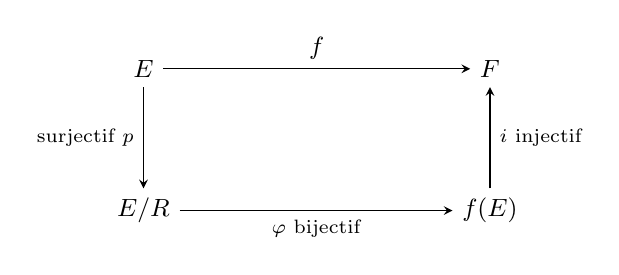
\begin{tikzpicture}[>=stealth, every node/.style={font=\small}]
\node (E) at (0,1.8) {$E$};
\node (F) at (4.4,1.8) {$F$};
\node (ER) at (0,0) {$E/R$};
\node (fE) at (4.4,0) {$f(E)$};
\draw[->] (E) -- node[above] {$f$} (F);
\draw[->] (E) -- node[left] {\scriptsize surjectif $p$} (ER);
\draw[->] (ER) -- node[below] {\scriptsize $\varphi$ bijectif} (fE);
\draw[->] (fE) -- node[right] {\scriptsize $i$ injectif} (F);
\end{tikzpicture}
\end{center}

avec $f=i\circ\varphi\circ p$. En effet, soit $x$ dans $E$, et $\mathcal X=p(x)$ sa classe, on a $\varphi(p(x))=f(x)$, car on peut prendre $x$ comme représentant de $\mathcal X$, d'où
\[
(i\circ\varphi\circ p)(x)=i(f(x))=f(x)\text{ vu la définition de }i.\quad\bookend
\]

\medskip\noindent\textsc{Théorème 2.40.} --- \emph{Soit un morphisme $f$ de $E$ dans $F$, $R$ l'équivalence d'application associée à $f$. Il existe un morphisme surjectif $p$ de $E$ sur $E/R$, un isomorphisme $\varphi$ de $E/R$ sur $f(E)$ et un morphisme injectif $i:f(E)\to F$ tels que $f=i\circ\varphi\circ p$.}

On a « décomposé canoniquement » $f$, comme nous venons de le justifier.

\BellaSection{5. Un morceau de choix : Zorn \texorpdfstring{$\Leftrightarrow$}{⇔} choix \texorpdfstring{$\Leftrightarrow$}{⇔} Zermelo}

Tout ce qui précède ressemble à un aimable bavardage : quelques axiomes logiques qui ne posent pas problème, et des raisonnements faciles. On va maintenant s'intéresser à un axiome d'un autre type qui sert \BellaCorrection{entre autres}{entre autre} pour justifier l'existence des bases dans les espaces vectoriels de dimension infinie, et l'existence des solutions dites maximales, pour les équations différentielles : c'est l'axiome dit de Zorn, qui peut se formuler de différentes façons.

D'abord du vocabulaire.

\subsection*{2.41.}
Un ensemble ordonné $E$ est dit \emph{inductif} si toute partie $C$, totalement ordonnée, de $E$ admet au moins un majorant. On a alors :

\subsection*{2.42. Axiome de Zorn}
\emph{Tout ensemble non vide, ordonné, inductif admet au moins un élément maximal.}

\subsection*{2.43.}
On appelle \emph{bon ordre} sur un ensemble $E$, toute relation d'ordre sur $E$ telle que toute partie non vide de $E$ admet un plus petit élément. Il est à remarquer qu'un bon ordre est forcément total, car pour une paire $\{a,b\}$ de $E$, comme il y a un plus petit élément, si c'est $a$, alors $a\le b$, et si c'est $b$, on aura $b\le a$. Dans les 2 cas, $a$ et $b$ sont comparables.

On énonce :

\subsection*{2.44. Axiome de Zermelo}
\emph{Tout ensemble $E$ non vide, peut être bien ordonné.}

Ainsi que :

\subsection*{2.45. Axiome du choix}
\emph{Pour tout ensemble non vide $E$, il existe au moins une application $f$ de $\mathcal P(E)$ dans $E$ telle que $\forall A\subset E$, avec $A\ne\varnothing$, on ait $f(A)\in A$.}

Donc $f$ est une « fonction de choix » qui permet de choisir un élément $a$ dans $A$ non vide.

L'axiome du choix, semble formaliser la phrase de bon sens suivante « soit $a$ dans $A$ », avec $A$ partie non vide de $E$. Il ressemble donc à l'un des axiomes logiques du départ de la théorie (cf. Chapitre 0). Il n'en est pas de même des 2 autres, moins intuitifs or... ils sont équivalents.

\medskip\noindent\textsc{Théorème 2.46.} --- \emph{Les axiomes de Zorn, de Zermelo et du choix sont équivalents.}

\subsection*{2.47. Zermelo $\Rightarrow$ choix}
Soit $E$ non vide, par Zermelo on le munit d'un bon ordre, donc si $A$ est une partie non vide de $E$, on sait que $A$ admet un plus petit élément $a$ : on pose $f(A)=a$. On définit ainsi $f$ sur $\mathcal P(E)-\{\varnothing\}$, avec $\forall A\in\mathcal P(E)-\{\varnothing\}$, $f(A)\in A$. Il suffit de définir $f(\varnothing)$ de manière quelconque, ($f(\varnothing)=f(E)$ par exemple) pour avoir une fonction de choix $f:\mathcal P(E)\to E$. \bookend

Pour justifier Zorn $\Rightarrow$ Zermelo, on va d'abord considérer les parties de $E$ que l'on peut munir d'un bon ordre, et montrer que leur ensemble est inductif.

\subsection*{2.48.}
Soit un ensemble non vide $E$, on considère l'ensemble $\mathcal M$ des couples $(A,O_A)$ où $A$ est une partie non vide de $E$ et $O_A$ un bon ordre sur $A$.

\subsection*{2.49.}
$\mathcal M\ne\varnothing$, car si $A$ est une partie de $E$ de cardinal fini, $n$ ; il existe une bijection $\varphi$ de $\{1,2,\ldots,n\}$ sur $A$, on peut donc noter $a_1=\varphi(1)$, $a_2=\varphi(2)$, ..., $a_n=\varphi(n)$ les éléments distincts de $A$ et ordonner $A$ par $O_A$ défini par
\[
a_p\,O_A\,a_q\Leftrightarrow p<q :
\]
c'est un bon ordre, l'élément le plus petit d'une partie étant celui associé à l'entier le plus petit. \bookend

Bien sûr, la notion de cardinal, et celle de cardinal fini ne font intervenir aucun des 3 axiomes précédents. D'ailleurs on peut se contenter de $n=1$ ou $2$, notions premières de notre théorie mathématique.

\subsection*{2.50.}
L'ensemble $\mathcal M$ peut lui-même être ordonné par la relation suivante : on dira que
\[
(A,O_A)\preccurlyeq(B,O_B)
\Leftrightarrow
\begin{cases}
1)\ A\subset B,\\
2)\ O_A\text{ est la restriction de }O_B\text{ à }A\times A,\\
3)\ A\text{ est partie héréditaire de }B.
\end{cases}
\]
Le 2) signifie que $\forall(x,y)\in A^2\subset B^2$, dire que $xO_Ay\Leftrightarrow xO_By$. Quant au 3), il signifie que, s'il existe $a\in A\subset B$, et $b\in B$, avec $bO_Ba$, alors $b\in A$ : en quelque sorte $A$ « hérite » des éléments de $B$ qui sont plus petits que des éléments de $A$, dans l'ordre $O_B$.

On a bien une relation d'ordre \BellaCorrection{sur $\mathcal M$}{M}, c'est-à-dire une relation réflexive, \BellaCorrectionNote{antisymétrique}{symétrique}{Une relation d'ordre est réflexive, antisymétrique et transitive ; la démonstration qui suit est d'ailleurs explicitement intitulée « Antisymétrie ».} et transitive.

\emph{Réflexivité :}
\[
(A,O_A)\preccurlyeq(A,O_A)\quad\text{car}\quad
\begin{cases}
1)\ A\subset A,\\
2)\ O_A\text{ est bien }O_A\text{ restreint à }A\times A,\\
3)\ A\text{ n'a aucun mal à hériter des éléments de }A.
\end{cases}
\]

\emph{Antisymétrie :} si $(A,O_A)\preccurlyeq(B,O_B)$ et $(B,O_B)\preccurlyeq(A,O_A)$, on a déjà $A\subset B$ et $B\subset A$ d'où $A=B$, puis l'ordre $O_A$ c'est l'ordre $O_B$ car $\forall(u,v)\in A^2=B^2$, comme $O_A$ est la restriction de $O_B$ à $A\times A$ on a
\[
uO_Av\Leftrightarrow uO_Bv :\quad\text{d'où }O_A=O_B.
\]

\emph{Enfin la relation est transitive :} si $(A,O_A)\preccurlyeq(B,O_B)$ et $(B,O_B)\preccurlyeq(C,O_C)$ on a $A\subset B$ et $B\subset C$ d'où $A\subset C$ ; puis $\forall(u,v)\in A^2\subset B^2\subset C^2$ on a $uO_Av\Leftrightarrow uO_Bv$ car $O_A$ est la restriction de $O_B$ à $A^2$ ; mais $O_B$ étant lui-même la restriction de $O_C$ à $B^2$, comme $(u,v)\in B^2$, on a aussi
\[
uO_Bv\Leftrightarrow uO_Cv,
\]
d'où finalement $uO_Av\Leftrightarrow uO_Cv$ ce qui est la traduction de $O_A$ restriction de $O_C$ à $A^2$.

Enfin $A$ est partie héréditaire de $C$ car si $c$ de $C$ est tel qu'il existe $a\in A$ avec $cO_Ca$, comme $a\in A\subset B$, et que $B$ est héréditaire de $C$, on a déjà $c\in B$, car inférieur, pour $O_C$, à un élément, ici $a$, de $B$.

Mais alors, comme $c$ et $a$ sont dans $B$, que $O_B$ est la restriction de l'ordre $O_C$ à $B$ écrire $cO_Ca$, c'est écrire $cO_Ba$, avec $a\in A$, $c\in B$ et $A$ héréditaire dans $B$. On a donc $c\in A$, ce qu'on voulait. On a ainsi justifié le point 2.50. \bookend

\subsection*{2.51. L'ensemble $\mathcal M$, non vide, ainsi ordonné, est inductif}

Soit $\mathcal C=\{(A_i,O_{A_i})_{i\in I}\}$ une partie de $\mathcal M$ totalement ordonnée, on doit lui trouver un majorant, dans $\mathcal M$, pour l'ordre $\preccurlyeq$ de $\mathcal M$. C'est évident si $\mathcal C=\varnothing$, (car alors, pour $m$ quelconque de $\mathcal M$, on a bien, $\forall x\in\varnothing$, $x\preccurlyeq m$ puisqu'il n'y a rien à vérifier, car il n'y a pas de $x$ dans $\varnothing$).

On suppose donc $\mathcal C\ne\varnothing$, (c'est-à-dire $I\ne\varnothing$) et soit
\[
R=\bigcup_{i\in I}A_i.
\]
On ordonne $R$ comme suit. Soient $r$ et $r'$ dans $R$, et $i$ et $i'$ dans $I$ tels que $r$ soit dans $A_i$ et $r'$ dans $A_{i'}$. On a soit $(A_i,O_{A_i})\preccurlyeq(A_{i'},O_{A_{i'}})$, soit l'inégalité contraire, car $\mathcal C$ est totalement ordonnée.

Dans le 1\textsuperscript{er} cas : $A_i\subset A_{i'}$, mais alors $r$ et $r'$ sont tous les deux dans $A_{i'}$ sur lequel $O_{A_{i'}}$ est un bon ordre, (donc un ordre total) et on posera $rO_Rr'$ si $rO_{A_{i'}}r'$, ou bien $r'O_Rr$ si on a $r'O_{A_{i'}}r$ : en somme l'ordre $O_R$ correspond à $O_{A_{i'}}$. \emph{A priori}, cet ordre $O_R$ pourrait dépendre du choix de $i'$ tel que $r$ et $r'$ soient dans $A_{i'}$, mais il n'en est rien, car si on trouve un $i''\in I$ tel que $r$ et $r'$ sont dans $A_{i''}$, là encore comme $(A_{i'},O_{A_{i'}})$ et $(A_{i''},O_{A_{i''}})$ sont comparables pour $\preccurlyeq$ ordre de $\mathcal M$, l'un des deux ensembles $A_{i'}$ ou $A_{i''}$ contient l'autre et l'ordre sur le plus petit est la restriction de l'autre ; on a en même temps $rO_{A_{i'}}r'$ et $rO_{A_{i''}}r'$, (ou les inégalités opposées).

Donc la définition de $O_R$ \BellaCorrection{a}{à} un sens. Si vous suivez encore, (et là vous avez du mérite), il reste à justifier que $O_R$ est un bon ordre. Pour vérifier que c'est un ordre, on doit prendre 1, 2 ou 3 éléments de $R$ suivant qu'on justifie la réflexivité, l'antisymétrie ou la transitivité. Or, ayant $i_1,i_2,i_3$ dans $I$ associés aux 3 parties $A_{i_1},A_{i_2},A_{i_3}$ contenant chacune un élément, l'une des 3 contient les 2 autres, (toujours $\mathcal C$ totalement ordonnée) donc finalement nos 3 éléments sont dans un $A_i$ tel que $(A_i,O_{A_i})\in\mathcal C$, et $\mathcal C\subset\mathcal M$ ; $O_R$ coïncide alors avec la relation $O_{A_i}$ qui est bien relation d'ordre : d'où $O_R$ relation d'ordre. De plus c'est un ordre total car dès le départ on avait $rO_Rr'$ ou $r'O_Rr$.

C'est un bon ordre, car soit $S$ partie non vide de $R$, et $s$ dans $S$. Si ce n'est pas le plus petit élément de $S$, c'est que
\[
T=\{t;\ t\in S,\ tO_Rs\}
\]
est non vide.

Soit alors $t$ dans $T$. Tout ceci se passe, il ne faut pas l'oublier dans $R=\bigcup_{i\in I}A_i$. Il existe donc $i$ et $i'$ dans $I$ tels que $s\in A_i$ et $t\in A_{i'}$. De plus $(A_i,O_{A_i})$ et $(A_{i'},O_{A_{i'}})$ sont comparables. Si $(A_{i'},O_{A_{i'}})\preccurlyeq(A_i,O_{A_i})$, on a aussi $t\in A_i$, car alors $A_{i'}\subset A_i$. Sinon, $(A_i,O_{A_i})\preccurlyeq(A_{i'},O_{A_{i'}})$ mais alors on a $t\in A_{i'}$, $s\in A_i$ et $tO_Rs$, soit comme $t$ et $s$ sont dans ce cas tous les deux dans $A_{i'}$, $tO_{A_{i'}}s$ vu la définition de l'ordre $O_R$. Comme dans ce cas $A_i$ est héréditaire dans $A_{i'}$, on a encore $t\in A_i$.

Dans les 2 cas, on parvient à $t\in A_i$. Ceci est vrai pour tout $t$ de $T$, finalement $T\subset A_i$, ($A_i$ choisi tel que $s\in A_i$), mais $A_i$ est lui bien ordonné par $O_{A_i}$.

Si $m$ est le plus petit élément de $T$ pour l'ordre $O_{A_i}$, ($m$ existe car $O_{A_i}$ bon ordre), alors pour tout $\sigma\in S$, on a soit $\sigma O_Rs$, donc $\sigma\in T$ et alors $mO_R\sigma$, (car $m$ et $\sigma$ sont dans le $A_i$ contenant $s$, et sur $A_i$ les ordres $O_R$ et $O_{A_i}$ coïncident), soit $sO_R\sigma$ (car $O_R$ est total, comme déjà signalé), et comme $mO_Rt$ pour un $t$ de $T$, que $tO_Rs$ et que $sO_R\sigma$, par transitivité on a bien $mO_R\sigma$ : dans tous les cas on a $mO_R\sigma$, donc $m$ est plus petit élément de $S$ partie non vide de $R$, donc $(R,O_R)\in\mathcal M$.

Je ne sais pas si quelqu'un suit encore... Enfin, faisons comme si...

La partie $\mathcal C=\{(A_i,O_{A_i})_{i\in I}\}$ est alors majorée par $(R,O_R)$ élément de $\mathcal M$ car, $\forall i_0$, $A_{i_0}\subset R=\bigcup_{i\in I}A_i$ ; par construction, $O_{A_{i_0}}$ est bien la restriction à $A_{i_0}\times A_{i_0}$ de $O_R$ ; et $A_{i_0}$ est héréditaire dans $R$ : si $x\in A_{i_0}$, $y\in R$, avec $yO_Rx$, il existe $i\in I$ avec $y\in A_i$, on a soit $(A_{i_0},O_{A_{i_0}})\preccurlyeq(A_i,O_{A_i})$ et alors $A_{i_0}$ héréditaire dans $A_i$ et $O_R$ coïncide avec $O_{A_i}\Rightarrow y\in A_{i_0}$ ; soit
\[
(A_i,O_{A_i})\preccurlyeq(A_{i_0},O_{A_{i_0}})
\]
et alors $y\in A_{i_0}$.

Dans les 2 cas, $y\in A_{i_0}$. On a ainsi justifié 2.51. \bookend

\subsection*{2.52. Zorn $\Rightarrow$ Zermelo}

En effet, $\mathcal M$ inductif, admet un élément maximal disons $(U,O_U)$. Si $U\ne E$, soit $x\in E-U$, $V=U\cup\{x\}$ muni de la relation d'ordre, (à justifier) $O_V$ définie par $\forall y\in V$, $yO_Vx$ et $\forall(y,y')\in U^2$, on pose
\[
yO_Vy'\Leftrightarrow yO_Uy'.
\]
On définit bien un bon ordre.

\emph{Réflexivité}, car $x\in V\Rightarrow xO_Vx$, et si $y\in U$, $yO_Uy$ donc $yO_Vy$.

\emph{Antisymétrie :} si on a $yO_Vy'$ et $y'O_Vy$ avec $y$ et $y'$ tous deux dans $U$, c'est qu'on a les inégalités $yO_Uy'$ et $y'O_Uy$ avec $O_U$ antisymétrique d'où $y=y'$ ; si $y$ ou $y'$ est égal à $x$ on n'est pas dans le cas $y$ et $y'$ dans $U$, c'est donc, vu la définition de $O_V$ que, si $y'=x$ par exemple, on ne peut écrire que $yO_Vx$, (avec impossibilité, si $y\ne x$, d'écrire $xO_Vy$) donc si on a aussi $xO_Vy$ c'est que $y=x$.

\emph{Transitivité :} soit $yO_Vy'$ et $y'O_Vy''$. Si $y,y'$ et $y''$ sont dans $U$ où $O_V$ coïncide avec l'ordre $O_U$, la transitivité est justifiée.

Si l'un des éléments est $x$, si c'est $y''$, $yO_Vy''$ avec $y''=x$ est évident ; si $y'=x$, forcément $y''=x$, d'où encore $yO_Vy''$ ; si $y=x$, forcément $y'=x$, $y''$ aussi d'où encore $yO_Vx$.

C'est un bon ordre car une partie de $V$ est soit $\{x\}$, avec $x$ plus petit élément ; soit du type $A\cup\{x\}$ avec $A\subset U$, elle admet $a$, plus petit élément de $A$ (pour l'ordre $O_U$) comme plus petit élément pour $O_V$ car $aO_Vx$ ; soit contenue dans $U$, et alors elle admet un plus petit élément.

Enfin $(U,O_U)\preccurlyeq(V,O_V)$, (facile à vérifier) avec $U\ne V$ : on aurait un élément de $\mathcal M$ strictement supérieur à $(U,O_U)$ maximal : absurde.

Donc $U=E$ et $O_U$ est un bon ordre sur $E$ : on a bien justifié Zermelo. \bookend

\subsection*{2.53.}
Il reste à voir, s'il y en a qui suivent encore, que choix $\Rightarrow$ Zorn pour fermer la boucle. Pour cela on part de $E$ non vide muni de $f$ fonction de choix.

Soit $E$ ordonné non vide. Si $H$ est une partie de $E$ on note
\[
\overset{>}{H}=\{x;\ \forall h\in H,\ h<x\}.
\]
Donc $\overset{>}{H}$ est formé des majorants de $H$, non dans $H$.

\medskip\noindent\textsc{Définition 2.54.} --- \emph{On appelle chaîne de $E$ ordonné, toute partie $K$ totalement ordonnée, par l'ordre de $E$. On appelle $k$-chaîne de $E$ toute chaîne $K$ non vide telle que toute partie $H$ héréditaire de $K$ et distincte de $K$ vérifie : $f(\overset{>}{H})$ est le plus petit élément de $\overset{>}{H}\cap K$.}

Qu'est-ce que cela veut dire ! D'abord, $f$ est la fonction de choix supposée exister.

$H\subset K$ est partie héréditaire de $K\Leftrightarrow$ tout $k$ de $K$, inférieur à un $h$ de $H$ est dans $H$.

Il en résulte que si $x\in K-H$, il ne peut pas être « hérité » par $H$ donc $\nexists h\in H$ avec $x<h$ : comme la chaîne $K$ est une partie totalement ordonnée, $x$ et $h$ sont comparables et $\ne$ car $x\notin H$, c'est que $h<x$.

Ceci est vrai $\forall h\in H$ donc $x\in\overset{>}{H}$ : on a $(K-H)\subset\overset{>}{H}\cap K$, mais si $x\in K\cap\overset{>}{H}$, il est dans $K$, pas dans $H$ par définition de $\overset{>}{H}$, d'où $x\in(K-H)$ et finalement on a :

\begin{description}[leftmargin=7.2em,labelwidth=6.4em,labelsep=.6em,font=\itshape]
\item[1\textsuperscript{er} point :] Si $H$ est une partie héréditaire de $K$, distincte de $K$, on a
\[
\overset{>}{H}\cap K=K-H.
\]
En particulier $\overset{>}{H}$ est non vide, donc $f(\overset{>}{H})$ existe, avec $f$ fonction de choix qui est supposée exister sur $E$ puisque, ne l'oublions pas, nous sommes en train de justifier choix $\Rightarrow$ Zorn.

\item[2\textsuperscript{e} point :] Il existe des $k$-chaînes.

En effet, soit $E$ non vide, muni d'une fonction de choix $f$, et $e=f(E)$. Alors $K=\{e\}$ est totalement ordonné, (par l'ordre $e\le e$ induit par celui sur $E$) de plus la seule partie $H$ distincte de $\{e\}$ c'est $\varnothing$, qui est héréditaire car la condition : soit $k\in K$ tel que $\exists h\in\varnothing$ avec $k\le h$... n'est jamais remplie, donc la conclusion $k\in\varnothing$ ne se présente jamais.

On a
\[
\overset{>}{\varnothing}\cap K=E\cap K=K,
\qquad
f(\overset{>}{\varnothing})=f(E)=e
\]
est le seul élément de $\overset{>}{\varnothing}\cap K=K=\{e\}$ donc c'en est bien le plus petit élément.

On a $\{e\}$ est une « $k$-chaîne ».

\item[3\textsuperscript{e} point :] Toutes les « $k$-chaînes » ont $e$ pour plus petit élément.

Car si $K$ est une « $k$-chaîne », comme $\varnothing$ est partie héréditaire de $K$ (cela vient d'être vérifié, et comme il n'existe jamais de $x$ dans $\varnothing$, supérieur à un $y$ de $K$, $\varnothing$ n'hérite jamais de l'élément $y$...) on a
\[
\overset{>}{\varnothing}\cap K=E\cap K=K,
\]
donc $e=f(\overset{>}{\varnothing})$ est plus petit élément de $\overset{>}{\varnothing}\cap K=K$.

\item[4\textsuperscript{e} point :] L'ensemble $\mathcal K$ des $k$-chaînes est totalement ordonné par inclusion et toute $k$-chaîne est héréditaire dans toute $k$-chaîne la contenant.
\end{description}

Pour justifier ce point, plus délicat, on introduit la notation suivante : si $x\in E$, on note
\[
\overset{\le}{x}=\{y;\ y\in E,\ y\le x\}.
\]

Soient $K_1$ et $K_2$ deux $k$-chaînes et
\[
I=\{x;\ x\in K_1\cap K_2;\ K_1\cap\overset{\le}{x}=K_2\cap\overset{\le}{x}\} :
\]
on va prouver que $I=K_1$ ou $K_2$, comme $I\subset K_1\cap K_2$ on aura alors $K_1\subset K_1\cap K_2$ donc $K_1\subset K_2$, ou $K_2\subset(K_1\cap K_2)$ et $K_2\subset K_1$. Donc $\mathcal K$ sera totalement ordonné par inclusion.

Toutes les $k$-chaînes ayant $e$ pour plus petit élément, $e\in K_1\cap K_2$ et forcément
\[
K_1\cap\overset{\le}{e}=\{e\}=K_2\cap\overset{\le}{e}
\]
donc $e\in I$.

$I$ est partie héréditaire de $K_1$ (et de $K_2$, par symétrie des rôles joués).

Car si on a $i\in I$ et $k_1\in K_1$ avec $k_1\le i$, $k_1\in\overset{\le}{i}$, mais alors
\[
k_1\in K_1\cap\overset{\le}{i}=K_2\cap\overset{\le}{i}
\]
donc $k_1\in K_2$ : on a déjà $k_1\in K_1\cap K_2$.

Puis
\[
(K_1\cap\overset{\le}{i})\cap\overset{\le}{k_1}
=(K_2\cap\overset{\le}{i})\cap\overset{\le}{k_1}.
\]
Mais
\[
\overset{\le}{i}\cap\overset{\le}{k_1}
=\{x;\ x\le i\text{ et }x\le k_1\},
\]
avec $k_1\le i$ il ne reste que la condition $x\le k_1$. On a $\overset{\le}{i}\cap\overset{\le}{k_1}=\overset{\le}{k_1}$ d'où l'égalité
\[
K_1\cap\overset{\le}{k_1}=K_2\cap\overset{\le}{k_1}.
\]
Ces deux résultats prouvent que $k_1\in I$ : $I$ a bien hérité du $k_1$ de $K_1$, avec $k_1\le i$.

On ne peut pas avoir à la fois $I\ne K_1$ et $I\ne K_2$ car alors, $I$ partie héréditaire de $K_1$, $k$-chaîne, et $I\ne K_1\Rightarrow m=f(\overset{>}{I})$ est le plus petit élément de $\overset{>}{I}\cap K_1$, mais pour la même raison, ($I\ne K_2$, $I$ héréditaire dans la $k$-chaîne $K_2$) on a aussi $m$ plus petit élément de $\overset{>}{I}\cap K_2$.

Comme $f$ est fonction de choix $m\in\overset{>}{I}$ : c'est un majorant de $I$, $m\notin I$, donc $I\subset\overset{<}{m}$, si on note
\[
\overset{<}{m}=\{x,\ x\in E,\ x<m\}.
\]
Par construction $I\subset K_1\cap K_2$, donc on aurait $I\subset K_1\cap\overset{<}{m}$.

Comme $m$ est le plus petit élément de $\overset{>}{I}\cap K_1$ ; c'est le plus petit élément qui soit à la fois dans $K_1$ et majorant strict de $I$, si bien que si $k\in K_1\cap\overset{<}{m}$, étant dans $K_1$ et strictement plus petit que $m$, il n'est pas majorant strict de $I$ donc $\exists i_0\in I$ avec $k\le i_0$. Mais $I$ est héréditaire dans $K_1$ donc $k\in I$ : on vient de prouver que $K_1\cap\overset{<}{m}\subset I$ d'où l'égalité
\[
I=K_1\cap\overset{<}{m},
\]
on aurait de même $I=K_2\cap\overset{<}{m}$.

Mais alors
\[
(K_1\cap\overset{<}{m})\cup\{m\}
=(K_1\cup\{m\})\cap(\overset{<}{m}\cup\{m\}),
\]
or $m$ plus petit élément de $\overset{>}{I}\cap K_1$ est dans $K_1$, donc il reste
\[
K_1\cap\overset{\le}{m}.
\]
Comme $K_1\cap\overset{<}{m}=K_2\cap\overset{<}{m}=I$, on obtient aussi
\[
(K_2\cap\overset{<}{m})\cup\{m\}=K_2\cap\overset{\le}{m}.
\]

On obtient donc $m\in K_1\cap K_2$ et
\[
K_1\cap\overset{\le}{m}=K_2\cap\overset{\le}{m},
\]
c'est donc que $m\in I$, (les 2 conditions sont vérifiées) or $m\in\overset{>}{I}$ est majorant strict de $I$ donc $m\notin I$ : c'est absurde (ouf !). Donc l'hypothèse $(I\ne K_1)$ et $(I\ne K_2)$ est absurde. On a par exemple $I=K_1$ soit $K_1\subset K_1\cap K_2$, d'où $K_1\subset K_2$ et $I$, ($=K_1$), héréditaire dans $K_2$. C'est la justification du 4\textsuperscript{e} point qui s'achève. \bookend

Soit alors
\[
K^*=\bigcup_{K\in\mathcal K}K,
\]
la réunion de toutes les $k$-chaînes.

C'est encore une $k$-chaîne. D'abord $K^*$ est une chaîne, (i.e. totalement ordonnée) car 2 éléments de $K^*$ sont \emph{a priori} dans deux $k$-chaînes $K_1$ et $K_2$ mais le 4\textsuperscript{e} point dit que l'une contient l'autre, donc nos 2 éléments sont dans une $k$-chaîne, qui est totalement ordonnée : ils sont comparables.

Puis si $H$ est une partie héréditaire de $K^*$, \BellaCorrection{distincte}{distinctes} de $K^*$, on veut prouver que
\[
s=f(\overset{>}{H})
\]
est le plus petit élément de $\overset{>}{H}\cap K^*$ (toujours avec $f$, fonction de choix sur $E$ du départ).

Soit donc $k\in\overset{>}{H}\cap K^*$, comme $k\in K^*$, il existe une $k$-chaîne $K$ contenant l'élément $k$, et $k$ majore $H$ sans lui appartenir, (définition de $\overset{>}{H}$).

Soit alors $h\in H$, si on suppose que $h\notin K$, il existe une autre $k$-chaîne $K'$ de la famille $\mathcal K$, contenant $h$, or $\mathcal K$ est totalement ordonné par inclusion et $K'\subset K$ est exclu. Donc $K\subset K'$, et le 4\textsuperscript{e} point donne $K$ partie héréditaire dans $K'$, comme $h\notin K$, il ne peut pas y avoir d'élément de $K$ majorant $h$, (sinon $K$ hérite de $h$) donc $h$ supérieur à tout élément de $K$ : en particulier $h>k$, alors qu'on avait $k\in\overset{>}{H}$ et $h\in H$, donc $k>h$ : c'est absurde.

Donc $h\in K$ c'est-à-dire $H\subset K$. Or $K\subset K^*$, on a supposé $H$ héréditaire dans $K^*$, \emph{a fortiori} $H$ est héréditaire dans $K$, (si $k_1$ de $K$, donc de $K^*$ est tel que $k_1\le h_1$ avec $h_1\in H$, on a bien $k_1\in H$). Mais $H$ héréditaire dans la $k$-chaîne $K$, et $H\ne K$, (car $k\in\overset{>}{H}$, donc $k\notin H$, or $k\in K$), par définition de $k$-chaîne on a $f(\overset{>}{H})$ est le plus petit élément de $\overset{>}{H}\cap K$ soit en particulier
\[
s=f(\overset{>}{H})\le k\in\overset{>}{H}\cap K,
\]
on était parti de $k$ quelconque de $\overset{>}{H}\cap K^*$ : on a finalement $s=f(\overset{>}{H})$ plus petit élément de $\overset{>}{H}\cap K^*$.

Donc $K^*$ est une $k$-chaîne, et $\overset{>}{K^*}=\varnothing$, sinon
\[
K_1=K^*\cup\{f(\overset{>}{K^*})\}
\]
est formé de $K^*$ auquel on ajoute, par la fonction de choix, un élément pris dans $\overset{>}{K^*}$ supposé non vide, donc un élément strictement plus grand que ceux de $K^*$, d'où $K_1$ totalement ordonné, et si $H$ est partie héréditaire de $K_1$, distincte de $K_1$ ; c'est soit $H=K^*$, alors $f(\overset{>}{H})=f(\overset{>}{K^*})$ est bien le plus petit élément de
\begin{align*}
\overset{>}{H}\cap K_1
&=\overset{>}{K^*}\cap\bigl(K^*\cup\{f(\overset{>}{K^*})\}\bigr)\\
&=(\overset{>}{K^*}\cap K^*)\cup\bigl(\overset{>}{K^*}\cap\{f(\overset{>}{K^*})\}\bigr)\\
&=\varnothing\cup\{f(\overset{>}{K^*})\}=\{f(\overset{>}{K^*})\};
\end{align*}
soit $H\subset K^*$, et alors $H$ est héréditaire dans $K^*$ qui est une $k$-chaîne donc $f(\overset{>}{H})$ est le plus petit élément de $\overset{>}{H}\cap K^*$, donc aussi de
\begin{align*}
\overset{>}{H}\cap K_1
&=\overset{>}{H}\cap\bigl(K^*\cup\{f(\overset{>}{K^*})\}\bigr)\\
&=(\overset{>}{H}\cap K^*)\cup\bigl(\overset{>}{H}\cap\{f(\overset{>}{K^*})\}\bigr),
\end{align*}
or $\overset{>}{H}\cap\{f(\overset{>}{K^*})\}$ est un élément de $\overset{>}{K^*}$ donc il majore ceux $K^*$ : cela ne change pas le plus petit élément de $\overset{>}{H}\cap K^*$.

Mais alors $K_1$ serait un élément de $\mathcal K$ ; vu la définition de $K^*$, on aurait $K_1\subset K^*$. Or, par construction, $K^*\subsetneq K_1$ : c'est absurde.\footnote{\textbf{校勘：}Le texte imprimé porte « on aurait $K^*\subset K_1$ c'est absurde ». Cette inclusion est précisément celle donnée par la construction de $K_1$ et n'est pas contradictoire. L'appartenance $K_1\in\mathcal K$ impose au contraire $K_1\subset K^*$ puisque $K^*$ est la réunion de toutes les $k$-chaînes ; combinée à $K^*\subsetneq K_1$, elle donne la contradiction.} On a bien $\overset{>}{K^*}=\varnothing$.

Si on suppose alors que $E$ est inductif, comme $K^*$ est une partie totalement ordonnée de $E$ inductif, $K^*$ admet au moins un majorant $m$ dans $E$, or $\overset{>}{K^*}=\{$majorants stricts de $K^*\}$ est vide, donc $m\in K^*$, mais alors $m$ est maximal dans $E$ car s'il existait un $y$ dans $E$ avec $y>m$, $m$ majorant de $K^*$, on aurait $y$ majorant de $K^*$ et $y\notin K^*$, (sinon $m$ non majorant de $K^*$) donc $y\in\overset{>}{K^*}$ qui est vide. C'est exclu, donc $m$ maximal et, après bien du mal, on a justifié que l'axiome du choix $\Rightarrow$ l'axiome de Zorn.

Je ne sais pas si j'ai été clair, mais si vous avez compris la démonstration, tous les espoirs vous sont permis !

Si vous n'avez pas compris, vous pouvez vous consoler en pensant que vous êtes sain d'esprit !

Ce n'est pas par masochisme que j'ai tenu à rédiger une justification de ces équivalences mais par ce que je pense être de l'honnêteté intellectuelle. Très rapidement on travaille sur des espaces vectoriels de dimension infinie, où les propriétés, pour être justifiées, nécessitent l'emploi de l'axiome de Zorn. De même les relations d'ordre sur les cardinaux utilisent la notion de bon ordre. Or il me semble que l'intérêt de la formation mathématique est de former des individus qui ne « s'en laissent pas conter », qui ne se contentent pas d'affirmations non justifiées. J'ai donc \BellaCorrection{préféré}{préférer} rédiger ces pages rébarbatives, quitte à ce que le lecteur ne les lise pas.
